\documentclass[12pt,a4paper]{article}
\usepackage{geometry}
\geometry{left=2.5cm,right=2.5cm,top=2.0cm,bottom=2.5cm}
\usepackage[english]{babel}
\usepackage{amsmath,amsthm}
\usepackage{amsfonts}
\usepackage[longend,ruled,linesnumbered]{algorithm2e}
\usepackage{fancyhdr}
\usepackage{ctex}
\usepackage{array}
\usepackage{listings}
\usepackage{color}
\usepackage{graphicx}
\usepackage{url}
\usepackage{hyperref}
\hypersetup{hidelinks}
\usepackage{longtable}
\usepackage{booktabs}
\usepackage{amsmath}
\usepackage{listings}

\lstset{
    basicstyle=\ttfamily\small,
    frame=single,
    breaklines=true,
    postbreak=\mbox{\textcolor{red}{$\hookrightarrow$}\space},
    showstringspaces=false,
    commentstyle=\color{gray},
    keywordstyle=\color{blue}
}

\begin{document}

\title{智能计算体系结构Lab5实验报告}
\date{}

\author{
姓名:\textbf{卞卓航}~~~~~~
学号:\textbf{22373017}~~~~~~
}

\maketitle

\section{实验说明}

本次实验在Lab4的基础上,去除了对PL的模拟,改为了使用真实的PL进行实验实现,达成使用硬件完成矩阵乘法的目的。

完成了全部10个问题,其中问题10提出了3项可行的解决方案。

由于Vivado原始工程过于巨大(1G),无法上传到spoc,没有放在附件中。如果需要麻烦助教联系我再获取~

\section{实验目标}

\begin{itemize}
\item
  联合板上的PL和PS侧,使用硬件实现高效的矩阵乘法
\item
  基于原先的乘法单元MAC,补齐各种操作,实现有序的乘法功能
\end{itemize}

\section{实验原理}

以前历次实验的大融合,实现了一个NaiveTPU。

尽管Naive,但是这个TPU能实现在硬件上利用BRAM为存储介质实现矩阵乘法运算,是了不起的。

在硬件上实现的小优化,都是对软件运行速度的巨大提升。

\section{实验实现}

\subsection{问题一}

按照工程中的设置,BRAM\_FM64的输入端口限制为\(64 * 4096\),BRAM\_WM128的输入端口限制为\(128 * 8192\),转换为实际存储参数uint8的数量,即为:

\begin{itemize}
\item
  \(M * N \le 8 * 4096 = 32768\)
\item
  \(N * P \le 16 * 8192 = 131072\)
\end{itemize}

当M为8字对齐,P为16字对齐时,可以进行取等。

\subsection{问题二}

是足够的

对于硬件而言,其并不关心具体存储的神经网络究竟是哪一个,只关心BRAM中能否放下相应的参数矩阵。

在本实验中,神经网络输入的最大规模为:

\begin{longtable}[]{@{}lll@{}}
\toprule\noalign{}
参数 & MLP & LeNet \\
\midrule\noalign{}
\endhead
\bottomrule\noalign{}
\endlastfoot
Feature & (1, 784) & (784, 25) \\
Weight & (784, 100) & 400, 120 \\
\end{longtable}

因此,对于Feature和Weight而言,输入的最大uint8参数数量为:

\begin{itemize}
\item
  \(Feature_{max} = 784 * 25 = 19600\)
\item
  \(Weight_{max} = 784 * 100 = 78400\)
\end{itemize}

对于存储Feature的BRAM\_FM32,其最大可以存储\(8 * 8192 = 65536 \ge 19600\)

对于存储Weight的BRAM\_WM32,其最大可以存储\(8 * 32768 = 262144 \ge 78400\)

因而均是足够的

\subsection{问题三}

实现覆盖率更强、更为自动化的随机测试

\subsubsection{思路概述}

修改TB主要分为以下几个部分:

\begin{enumerate}
\item
  删除原先从文件中读取参数的方法
\item
  在initial块中进行随机化,并重复进行测试
\end{enumerate}

修改TB为工程文件中的\texttt{MM\_top\_tb\_random.v}。在此简要描述一下修改的思路:

\begin{enumerate}
\item
  删去原先从文件中读取数据的方式,改为由\texttt{\$random}进行生成
\item
  修改数据的产生方式:原先的数据逻辑为进行两轮test,分别使用testcase1和testcase2中的数据进行测试。现在修改所有参数均为随机生成,且进行多轮测试
\item
  修改控制信号的控制逻辑:原先的控制只进行两轮,现在进行多轮测试。只要达到\texttt{c\_state==IDLE}状态,即可进行下一轮新的测试
\item
  在完成后,进行结果比对,结果正确则进行下一轮,否则使用仿真的系统函数\texttt{\$finish}结束仿真
\end{enumerate}

\subsubsection{实验思路}

\paragraph{逻辑控制部分}

主要修改了状态转移部分,使得在相应状态后进行数据赋值、结果检验等操作。

为了进行数据赋值操作,新设立了feature和weight两个变量,用于保存生成的值。

同时,基于原有的控制信号,在每次检验到\texttt{c\_state\_f3\ ==\ READ\_OUT}后,说明乘法器输出了一个数据,对数据进行保存:

\begin{lstlisting}
// 记录计算结果
always @(posedge arm_clk) begin
  if (c_state_f3 == READ_OUT) begin
    result_sim[result_cnt] = arm_BRAM_OUT_douta;
    //$display("[%d]: %d", result_cnt, result_sim[result_cnt]);
    result_cnt = result_cnt + 1;
  end
end
\end{lstlisting}

基于此,可以将数据进行保存,在后续对数据进行检验。

\paragraph{数据生成逻辑}

利用\texttt{\$random}生成逻辑,同时对边界值进行一定的处理。Feature和Weight的生成思路是一致的,这里简单摘取Feature的生成逻辑:

\begin{lstlisting}  
{FM_reg0, FM_reg1, FM_reg2, FM_reg3} = $random;
// 处理边界情况
if(i + 1 >= M) begin
    FM_reg1 = 0;
    FM_reg2 = 0;
    FM_reg3 = 0;
end 
else if(i + 2 >= M) begin
    FM_reg2 = 0;
    FM_reg3 = 0;
end 
else if(i + 2 >= M) begin
    FM_reg3 = 0;
end

// 记录生成值
feature[i  ][j] = FM_reg0;
feature[i+1][j] = FM_reg1;
feature[i+2][j] = FM_reg2;
feature[i+3][j] = FM_reg3;
\end{lstlisting}

值得注意的是,这里对边境情况进行了清零处理。

\paragraph{结果检验}

检验的逻辑很简单,在计算完成,即\texttt{c\_state\ ==\ FINISH}且生成了\texttt{M*P}个数据后,按照矩阵乘法的定义进行检验:

\begin{lstlisting}
for(i = 0; i < M; i = i + 1) begin
  for(j = 0; j < P; j = j + 1) begin
      result_std = 'b0;
      for(k = 0; k < N; k = k + 1) begin
          result_std = result_std + $signed(weight[k][j]) * $signed({8'b0, feature[i][k]});
      end
      if(result_sim[i*P+j] != result_std) begin
          error_flag = 1'b1;
      end
  end
end
\end{lstlisting}

在\texttt{error\_flag}为真,即出错时,使用系统函数\texttt{\$finish},直接退出仿真,减少不必要的损耗。

\subsubsection{实验效果}

达到的效果截图:

TCL-Console截图为:

\begin{figure}[htbp]
    \centering
    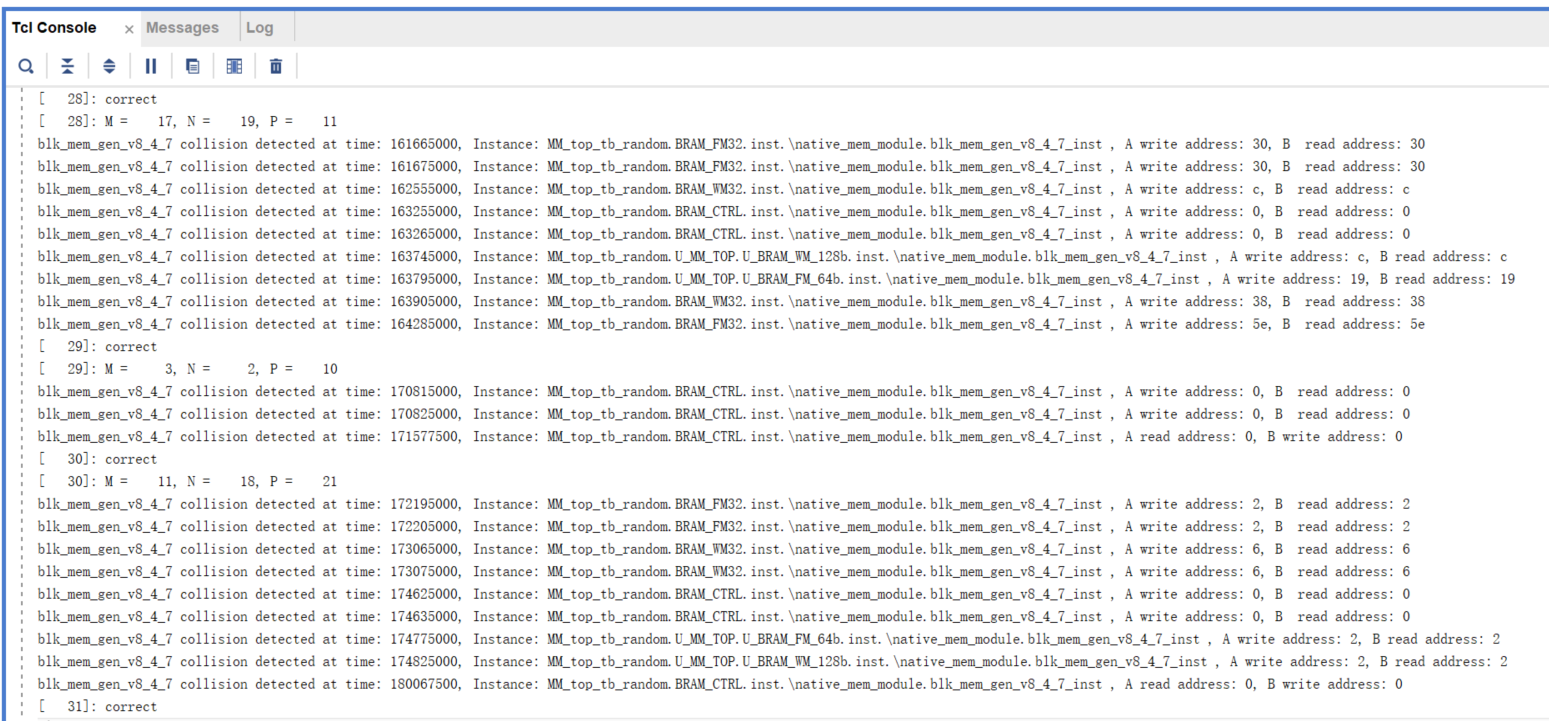
\includegraphics[width=\linewidth]{img/TCL.png}
    \caption{TCL-Console}
\end{figure}

仿真波形截图为:

\begin{figure}[htbp]
    \centering
    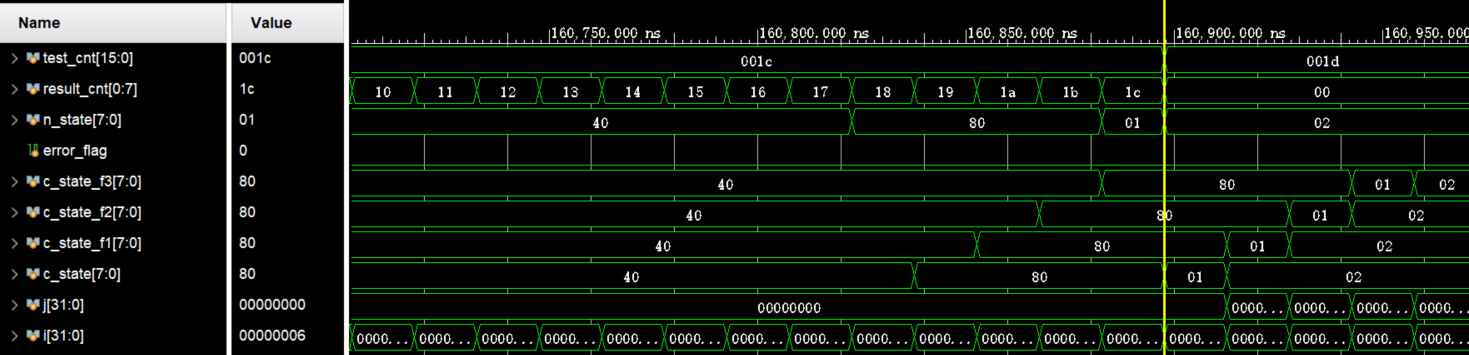
\includegraphics[width=\linewidth]{img/wave.png}
    \caption{Wave}
\end{figure}

工程文件的修改主要在于\texttt{Multiply\_ctrl}中,对获取数据的方式进行了修改,由原先的

\subsubsection{Matmul中的修改}

PS侧的数据直接写到BRAM\_FM\_32b和BRAM\_WM\_32b中,与原先统一写到BRAM\_32中的方式不同,故补0方式也不同。

和原先的相比,主要修改了\texttt{\_zero\_padding}中对补0的步长

将原先的统一补0为\texttt{uint8}形式调整为了:

\begin{itemize}
\item
  当为Feature矩阵时,按照步长为8进行补0
\item
  当为Weight矩阵时,按照步长为16进行补0
\end{itemize}

这实际上也是根据矩阵分块的性质进行的调整

\subsubsection{运行结果}

可以看到如下的结果,说明计算结果正确:

\begin{figure}[htbp]
    \centering
    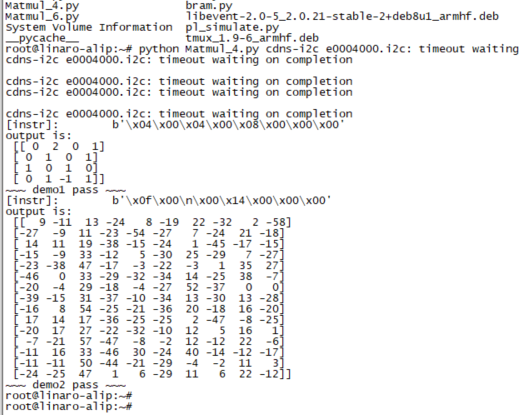
\includegraphics[width=0.6\linewidth]{img/result_4.png}
    \caption{result 4}
\end{figure}

\subsection{问题五}

补零是不必要的。原因分析见下。

\subsubsection{原因}

即使不补充,在PL侧的数据搬运过程中也会填充相应的0数据,以达到矩阵粉块的作用。

在PL侧的补0操作并不是根据BRAM中的已有数据决定的,而是根据矩阵的参数MNP决定的,故补充什么数据在PL侧看来是不重要的,在\textbf{模拟PL}侧看起来是重要的。

\subsubsection{PL侧补0的操作}

PL侧补0的操作涉及到了Feature矩阵和Weight矩阵,由于BRAM的大小不同,故补0的操作也不同。

对于Feature矩阵:

\begin{lstlisting}
// 对BRAM_FM64写入的数据
always @(posedge clk or posedge rst) begin
    else if (c_state == WORK) begin
        // 数据拼接,同时达到了补0的效果
        // 进行数据拼接,将32位数据合成64位数据
        // 先写入低位
        if (cycle1_cnt[0] == 1'b0)
            BRAM_FM64_wrdata <= {32'b0, BRAM_FM32_rddata};
        // 再写入高位
        else
            BRAM_FM64_wrdata <= {BRAM_FM32_rddata, BRAM_FM64_wrdata[31:0]};
    end
end

// 对BRAM_WM128写入的数据
always @(posedge clk or posedge rst) begin
    else if (c_state == WORK) begin
        // 数据拼接,同时达到了补0的效果
        case(cycle1_cnt[1:0])
            2'b00: BRAM_WM128_wrdata <= {96'b0, BRAM_WM32_rddata};
            2'b01: BRAM_WM128_wrdata <= {64'b0, BRAM_WM32_rddata, BRAM_WM128_wrdata[31:0]};
            2'b10: BRAM_WM128_wrdata <= {32'b0, BRAM_WM32_rddata, BRAM_WM128_wrdata[63:0]};
            2'b11: BRAM_WM128_wrdata <= {BRAM_WM32_rddata, BRAM_WM128_wrdata[95:0]};
            default: BRAM_WM128_wrdata <= BRAM_WM128_wrdata;
        endcase
    end
end
\end{lstlisting}

这里的补0操作利用了数据写入的时间先后顺序,实现对数据的补充。

\subsection{问题六}

\subsubsection{MAtmul中的修改}

由于进行了跳写,故可以不用对原始数据进行padding操作,而是直接在对应偏移量处直接写入数据。

核心在于每次对BRAM写入一行的数据,把所有的行进行写入。

\begin{lstlisting}
n, p = data.shape
p = p if p % self.systolic_size == 0 else (p // self.systolic_size + 1) * self.systolic_size

# C语言风格的内存布局:行优先
data = data.copy(order='C')

for i in range(n):
    self.bram.write(data[i], block_name=block_name, offset=i * p)
\end{lstlisting}

同时,需要注意对不满一行数据的特殊处理,并将数据按照行优先的方式进行排列。

\subsubsection{BRAM中的修改}

为了支持直接在offset处进行写操作,对\texttt{bram.py}文件中封装的\texttt{wrtie}函数进行修改,使得能够直接写对应offset处的数据。

\begin{lstlisting}
mem_offset = self.block_info[block_name]['offset'][offset] if isinstance(offset, str) else offset
\end{lstlisting}

\subsubsection{结果}

结果为:

\begin{figure}[htbp]
    \centering
    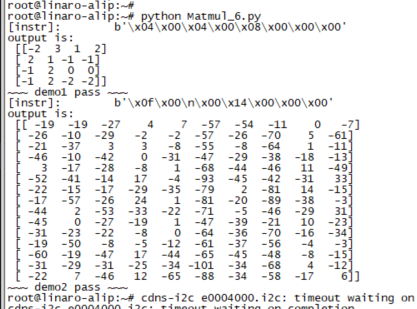
\includegraphics[width=0.6\linewidth]{img/result_6.png}
    \caption{result 6}
\end{figure}

\subsection{问题七}

频率为125MHz

FPGA侧即为PL侧,故可以查看PL中的相应时钟频率。

\begin{figure}[htbp]
    \centering
    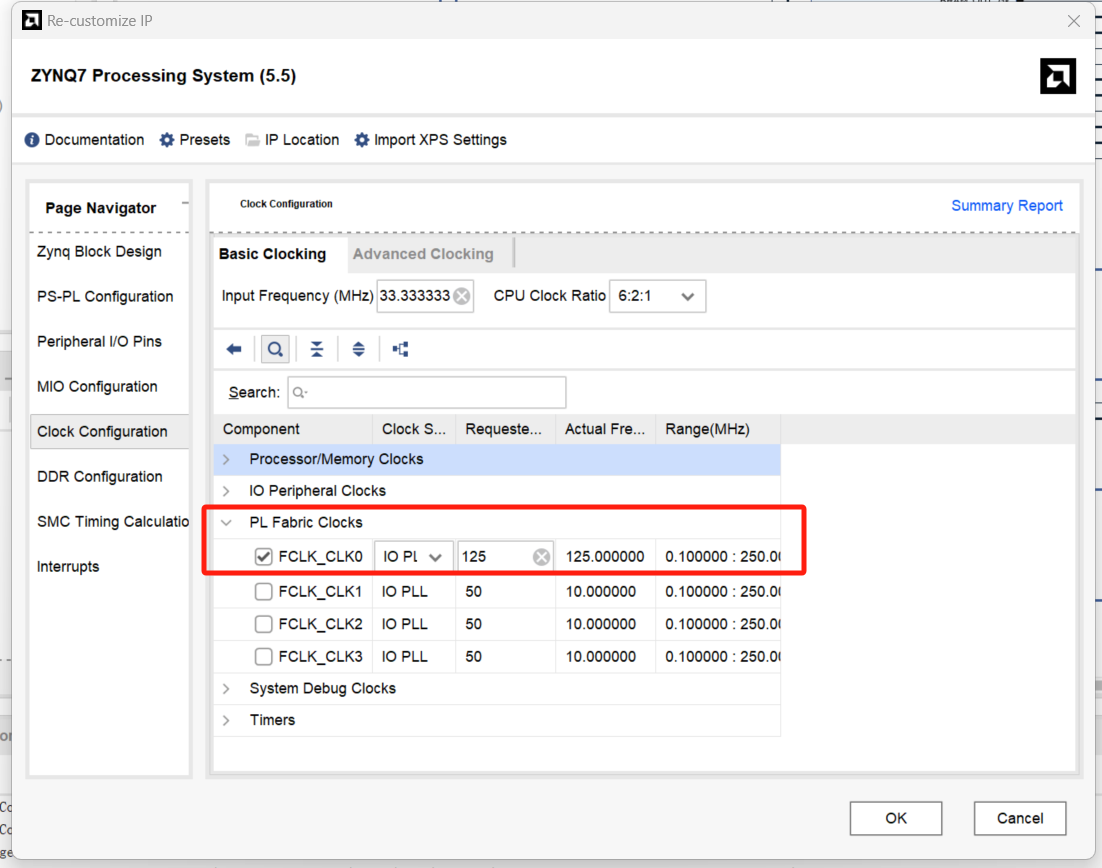
\includegraphics[width=0.6\linewidth]{img/f_7.png}
    \caption{时钟频率}
\end{figure}

\subsection{问题八}

\subsubsection{状态转移图}

首先需要明确各个状态的定义,参考指导书给以给出为:

\begin{longtable}[]{@{}ll@{}}
\toprule\noalign{}
名称 & 含义 \\
\midrule\noalign{}
\endhead
\bottomrule\noalign{}
\endlastfoot
IDLE & 初始状态 \\
INFO & 传递参数,项对齐结果的fifo传递需要对齐的矩阵参数 \\
WORK & 进行计算,本质是在向乘法器中搬运数据 \\
WAIT & 搬运数据完成后,乘法器会自动向对齐fifo传递数据,等待对齐完成 \\
FINISH & 完成所有计算 \\
\end{longtable}

可以得到状态转移图:

\begin{figure}[htbp]
    \centering
    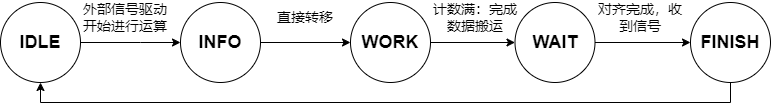
\includegraphics[width=0.8\linewidth]{img/dfa.png}
    \caption{状态转移图}
\end{figure}

\subsubsection{寄存器功能}

由于有两个乘法器进行运算,而只有一个控制器,所以需要两套参数来记录每个乘法器进行运算的参数信息。

第一套参数:记录在图中左侧乘法器和align-fifo所需要的参数

\begin{itemize}
\item
  \texttt{sub\_scale\_M1}:子矩阵1的M
\item
  \texttt{sub\_scale\_P1}:子矩阵1的P
\end{itemize}

第二套参数:记录在图中右侧乘法器和align-fifo所需要的参数

\begin{itemize}
\item
  \texttt{sub\_scale\_M2}:子矩阵2的M
\item
  \texttt{sub\_scale\_P2}:子矩阵2的P
\end{itemize}

对于M而言,其含义是结果矩阵的行数,而在乘法器中矩阵按行方向送入,故M代表了送入每个运算器、fifo寄存器的数据量,也可以说是循环数。有\texttt{sub\_scale\_M1\ =\ sub\_scale\_M2}

对于P而言,其含义是结果矩阵的列数,对于两个乘法器而言是不一样的,上限为8,故计算为:

\begin{lstlisting}
// 对齐M次
sub_scale_M1 <= sub_M;
sub_scale_M2 <= sub_M;
// 需要的对齐单元数,要考虑是否需要两个单元
sub_scale_P1 <= (sub_P > 'd8)? 'd8: sub_P;
sub_scale_P2 <= (sub_P > 'd8)? (sub_P - 'd8): 'd0;
\end{lstlisting}

\subsection{问题九}

下面将简单介绍IP单元、对齐流程、写过程和读过程。

\subsubsection{IP单元}

Aliogn-fifo使用了IP单元\texttt{U\_out\_align\_fifo}作为基本的Fifo单元,共有8个。

对于Fifo单元,其各接口的含义为:

\begin{lstlisting}
out_align_fifo U_out_align_fifo(
    .clk   (clk),
    // 写使能
    .wr_en (fifo_wr_en[i]),
    // 读使能:对fifo中的数据依次读出
    .rd_en (fifo_rd_en[i]),
    // 输入数据
    .din   (fifo_data_in[i]),
    // 输出数据
    .dout  (fifo_data_out[i]),
    // fifo是否满,空置
    .full  (),
    // fifo是否为空
    .empty (fifo_empty[i])
);
\end{lstlisting}

由于Fifo采用了先进先出的设计,故读使能还具有将数据送出的作用,这点比较独特

\subsubsection{对齐流程}

对齐流程实际上就是:

\begin{enumerate}
\item
  对于8个Fifo,依次读入数据,直到均读满数据
\item
  当8个Fifo均读满数据后,说明已经存入了全部的数据,由于之前没有送出数据,故已经有了对齐效果
\item
  将数据送出,达成对齐效果
\end{enumerate}

波形图为:

\begin{figure}[htbp]
    \centering
    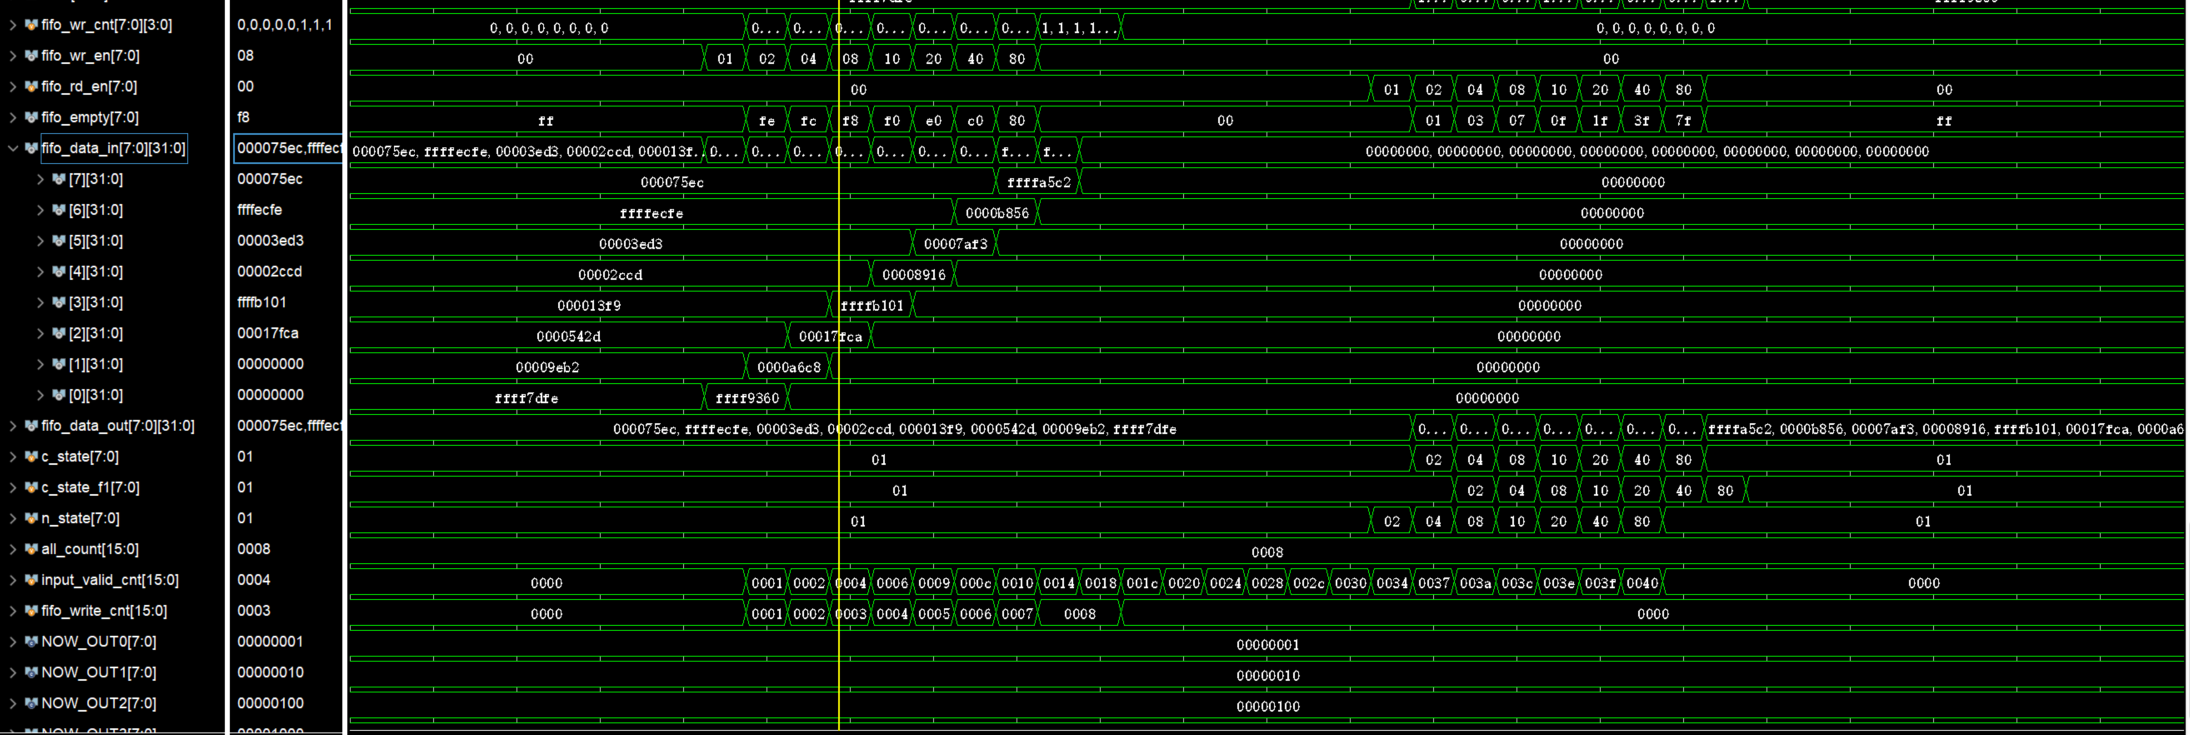
\includegraphics[width=0.8\linewidth]{img/wave_9.png}
    \caption{波形图}
\end{figure}

\subsubsection{写过程}

对于每一个Fifo,均有单独的写使能和数据输入进行控制。

当外部输入有效且\textbf{数据没有达到上限}时,即可进行读入。

\begin{lstlisting}
// 写使能
assign fifo_wr_en[0] = (~align_fifo_get_all) && valid_get0 && (sub_scale_P > 8'd0) && (fifo_wr_cnt[0] < sub_scale_M);
\end{lstlisting}

同时,之前的\texttt{Multiply\_ctrl}单元发送了结果矩阵的参数M、P,在写入数据过程中也会记录写入的数据数量没有超过限制。

\subsubsection{读过程}

Align-Fifo只有一个对外的输出,如何依次输出所有的数据:读过程是基于乘法器的数据输出特点,利用状态机实现的,每周期输出一个数据,依次从第一行输出到第八行。

对于状态机,即为简单的NOW\_OUT0\textasciitilde NOW\_OUT7,每周期转移至下一个数据列,同时也会检查相应的结果矩阵参数。

\begin{lstlisting}
case(c_state)
    NOW_OUT0: begin
        fifo_rd_en[0] = (~fifo_empty[0]) & out_ctrl_ready;
        valid = fifo_rd_en[0];
        data = fifo_data_out[0];
    end
endcase
\end{lstlisting}

利用状态机的特性,给予读使能和读数据选择,从而实现了有序输出。

\subsection{问题十}

以下介绍问题和实现思路,具体的工程文件见\texttt{question10}文件夹。

\subsubsection{削减 MAC 资源}

实现见文件。

\paragraph{问题}

原先的MAC设计存在大量的冗余控制信号:

\begin{itemize}
\item
  对于MAC之间的横向数据和纵向数据传递,分别使用了\texttt{w\_valid}和\texttt{f\_valid}信号
\item
  全局有一个\texttt{num\_valid}和\texttt{rst}信号
\end{itemize}

由于MAC固定的计算节奏,这样的控制信号设计是冗余没有必要的,可以进行删除代替。

\paragraph{实现}

由于MAC的数据传递固定为每个计算结点向右向下传递数据,故实际计算中的信号只需要确定计算的开始和结束,MAC单元会自动负责计算的进行。

并且,由于MAC中设计有了计算器,实际上每个MAC是清除自身的行为逻辑的,不需要额外的外部信号进行驱动,可以只使用一个外u开始有效信号\texttt{num\_valid}信号完成对于数据有效的控制,其效果为:

\begin{enumerate}
\item
  重置MAC内部寄存器,设置\texttt{num\_r}寄存器为输入的\texttt{num\_r}值
\item
  当输入数据有效时,拉低num\_valid信号,乘加器自动开始计数,在指定周期内完成乘法的运算要求
\end{enumerate}

可以将整个矩阵乘法器与外部对接的\texttt{num\_valid}信号接入左上角的第一个乘加模块,后续模块的\texttt{num\_valid}信号接入左侧或者上方乘加模块的\texttt{num\_valid\_r}输出。

由于MAC进行了大量的重复使用,简单的优化都可以带来较好的资源提升效果。

\subsubsection{输入输出对齐优化}

实现见文件。

\paragraph{问题}

尽管输入输出并不涉及计算时序,但是输入输出的数据搬运时序严重约束了操作。

且当前使用FIFO的设计有如下问题:为了使用IP核,造成了资源冗余,如使用的\texttt{U\_out\_align\_fifo},其中为了满足IP的使用约束有大量无意义的操作,如诡异的控制逻辑,大量冗余的控制信号。

实际上这样的操作是没有必要的,有如下几个原因:

\begin{enumerate}
\item
  实际上乘法模块的输出顺序是确定的,不存在中间结果的阻塞。确定的时许关系不需要冗余的握手信号
\item
  乘法器的数据输入宽度有限,最宽为8,完全可以替换为8列的寄存器序列,使用寄存器的时序效果进行对齐
\item
  由于输入的特性,可以较快完成输入,没必要使用完整的FIFO
\end{enumerate}

\paragraph{实现}

使用SystemVerilog实现了一个\texttt{my\_fifo.sv},使用寄存器队列代替原先的IP效果,实现了对数据的对齐。

对于输入:

\begin{itemize}
\item
  后一列/行的数据要求输入滞后前一列/樊的数据一个周期,因此对于每后一列,都可以加上一个寄存器,达到延缓的效果。
\item
  按照这种方式给每一列的数据输入加上不同级数的寄存器,就完成了数据的align操作,并不需要单独的fifo实现。
\end{itemize}

这样实现的对齐模块,可以有效的降低设计复杂度和资源占用情况,不再需要额外的Align-Fifo的IP,且易于实现参数化。

\subsubsection{参数化}

\paragraph{问题}

当前的设计限制了输入矩阵最多为\texttt{8*N,\ N*8},尽管使用了矩阵分块操作,但很可能还是不够用的。如进行浮点乘需要16位。为了解决此问题,可以使用语法中的参数功能进行优化,破除原先的固定大小。

当然,这样实现也是有限制的,如BRAM的地址空间约束等等。

由于实现此优化几乎无法用Verilog语言完成,需要使用SystemVerilog或Chisel等语言完成,需要重写整NativeTPU,由于相应的DDL的时间约束,这里仅提出方案思考,并没有实际解决。

\paragraph{实现}

方案为:

\begin{enumerate}
\item
  使用SystemVerilog进行一定重写:这两个语言绝大部分是相同的,SystemVerilog在Verilog基础上进行了一定的扩展,重写的额外花费是不大的
\item
  对数据的输入宽度、数据总线的传递进行参数化,使得其能支持\texttt{*parameter\ int*\ NUM\_WIDTH\ =\ 8}形式的模块参数化
\item
  对顶层的Vivado工程进行一定的修改,是得支持更大的BRAM地址空间,支持更灵活的数据操作
\end{enumerate}

\section{实验结果与分析}

取得了较好的实验效果。

可以使用硬件实现矩阵乘法:

\begin{figure}[htbp]
    \centering
    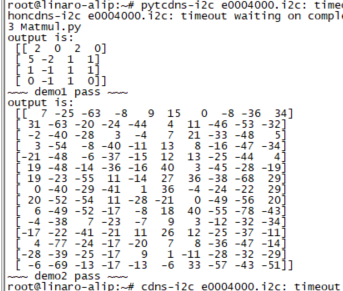
\includegraphics[width=0.6\linewidth]{img/result_result.png}
    \caption{实验结果}
\end{figure}

\section{实验总结}

使用硬件实现了良好的矩阵乘效果,将之前历次实验的结果进行了融合,达到了较好的效果。

在硬件上能实现的操作,都是对性能的巨大提升!

\end{document}
